\section{Introduction}
In the scope of compiler construction managed by Prof. Kirsch we implemented a compiler. The language we choose to compile is a subset of Java and the compiler itself is written in Java too. We implemented a single-pass compiler, a linker and a virtual machine for executing the generated output file. Figure \ref{components} shows the parts of our compiler. The main source of literature was the book ``Compiler Construction'' written by Nikolaus Wirth.
\paragraph{} Important design concepts:
\begin{itemize}
 \item We implemented a single-pass compiler, 
 \item a recursive descent parser 
 \item based on the RISC-Architecture defined in % TODO Wirth.
\end{itemize}
\subsection{Features}A brief overview of the features our compiler supports:
\begin{itemize}
\item modules
\item global hiding (implemented in modules)
\item methods (with parameters and return values)
\item local hiding (implemented in methods)
\item conditionals, loops
\item one-dimensional arrays
\item basic data types (boolean, int, char)
\item extended data types (modules)
\item separate compilation (linking)
\item syntax check (weak and strong error levels)
\item type safety
\item arithmetic and boolean operations
\item basic I/O operations
\end{itemize}


\subsection{Input language}
We decided to compile a LL(1) compliant subset of Java. The programming language is defined by EBNF, see \ref{labelEBNF}.
Listing \ref{example} shows any source file for our compiler.

\begin{lstlisting}[caption={Input language example},label={example}]
package examples;

import Util;

public class TestStuff {

	int a = 2;
	int[] b = int[9];
	
	public static void compare(int a, int b, char c) {

		int x = 0;
		int y = 1;
		if (((((a*20) > (b+b+1)) && (c == d)) && 
			(c == 'a')) || (c == 'a')) {
			println(x);
		} else {
			compare(a,b,'x');
		}
	}
	
	public static void main() {
		
		int b=6;
		int c=7;
		char x = 'a';

		compare(a,a,x,);
		Util.calc(a, b, c);
	}
}

package examples;

public class Util {
	
	public static void calc(int a, int b, int c) {
		int result = 2 + (3 + 4) * (a + 3 * ((3*b) * (4+c)));
		println(result);
	}
}
\end{lstlisting}

\subsection{Output language}
Our output language is based on the RISC architecture defined by Wirth. The Code Generator creates object files for the linker, the linker itself creates a output file for executing on the Virtual Machine. Both, the object and the execution file are binary files.

The binary file we execute on the Virtual Machine consist of a stream of operation code (3-address code). Each operation is represented by a 32 bit word. Thus our compiler is continuous word aligned and a word in ComPiler consists of 32 bit. 

\begin{figure}[h]
\label{components}
\begin{center}
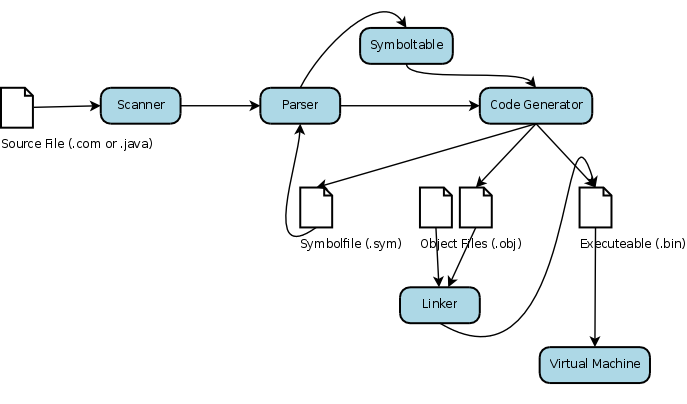
\includegraphics[width=13cm,height=7cm]{images/compParts.png}
\end{center}
\caption{Components of ComPiler}
\end{figure}


